\scanpage{132}
% archive sheet number: 131
Vérifions d) : $\forall\,a'\in X'$, le nb des $x\in X$ incidents à $a'$ est bien trois\ldots

a) Soient $a,b\in X$, \inserted{$a\ne b$,} considérons les $\underline t\in X'$ incidents à $a$ et $b$ à la fois, je dis qu'il y en a 0 ou 1 (jamais 2) : clair

b) Soient $\underline t,\underline t',\underline t''\in T=X'$ \inserted{él. distincts} et $a,b,c\in X$ tels que $\underline t,\underline t'$ incidents à $a$, $\underline t',\underline t''$ inc. à $b$, $\underline t'',\underline t$ inc. à $c$, prouver que $a=b=c$ donc que $\{\underline t,\underline t',\underline t''\}$ inc. à un \unsure{$=$|même} point\ldots En effet, si on avait $b\ne a$, le triangle $\underline t''$ ne pourrait rencontrer $\underline t$, car $b$ ne serait pas lié à un autre sommet de $\underline t$ que $a$.
\figure{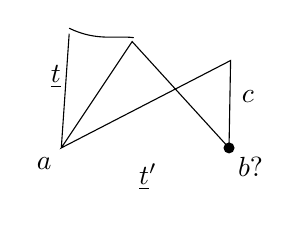
\begin{tikzpicture}
\draw (0,0)--(.1,1.45) (0.1,1.52).. controls (.45,1.35) and (.7,1.43)..(.92,1.4) (.9,1.35)--(0,0)--(2.15,1.11)--(2.13,0)--cycle;
\fill (2.13,0) circle (2pt);
\node[below left] at (0,0){$a$};\node[left] at (.12,.9){$\underline t$};\node[below] at (1.1,-.08){$\underline t'$};\node[right] at (2.17,.65){$c$};\node[below right] at (2.12,0){$b$?};
\end{tikzpicture}}

c) $\forall\,a\in X$ et $\underline t\in T=X'$\inserted{(\unsure{obs|PS|NB} $a$ n. incidt à $\underline t$)}, $\exists\,b\in X$ incident à $\underline t$, et tel que $a,b$ sont incidents à un $=$ $\underline t'\in T=X'$
\figure{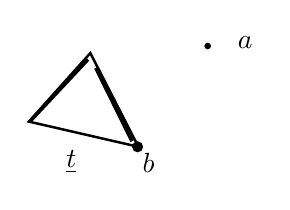
\begin{tikzpicture}
\draw[line width=.9pt] (0,0)--(.78,.87)--(1.39,-.32)--cycle;
\draw[line width=1.3pt] (.02,.01)--(.75,.79) (.85,.68)--(1.31,-.25);
\fill (1.38,-.32) circle(2pt) (2.27,.96) circle(1.2pt);
\node[right] at (2.53,1){$a$};\node[below] at (.54,-.24){$\underline t$};\node[below right] at (1.32,-.28){$b$};
\end{tikzpicture}}
